\documentclass{beamer}
\usepackage{graphicx}

\usetheme{Antibes}
\beamertemplatenavigationsymbolsempty
\title{Movement-based TV control}
\subtitle{Pervasive computing lab project}
\author{Franklin \textsc{Delehelle} \& Mario \textsc{Lassenberger}}
\date{}

\begin{document}

\begin{frame}
  \titlepage
\end{frame}
\section{What does it do?}
\begin{frame}
  \begin{itemize}
  \item Remotely control a TV through IR command
  \item Allows a simple and rustic priority and authorization system
  \item Offers a TCP interface for configuration or commands
  \end{itemize}
\end{frame}

\section{How does it works?}

\subsection{General overview}
\begin{frame}
  \begin{center}
    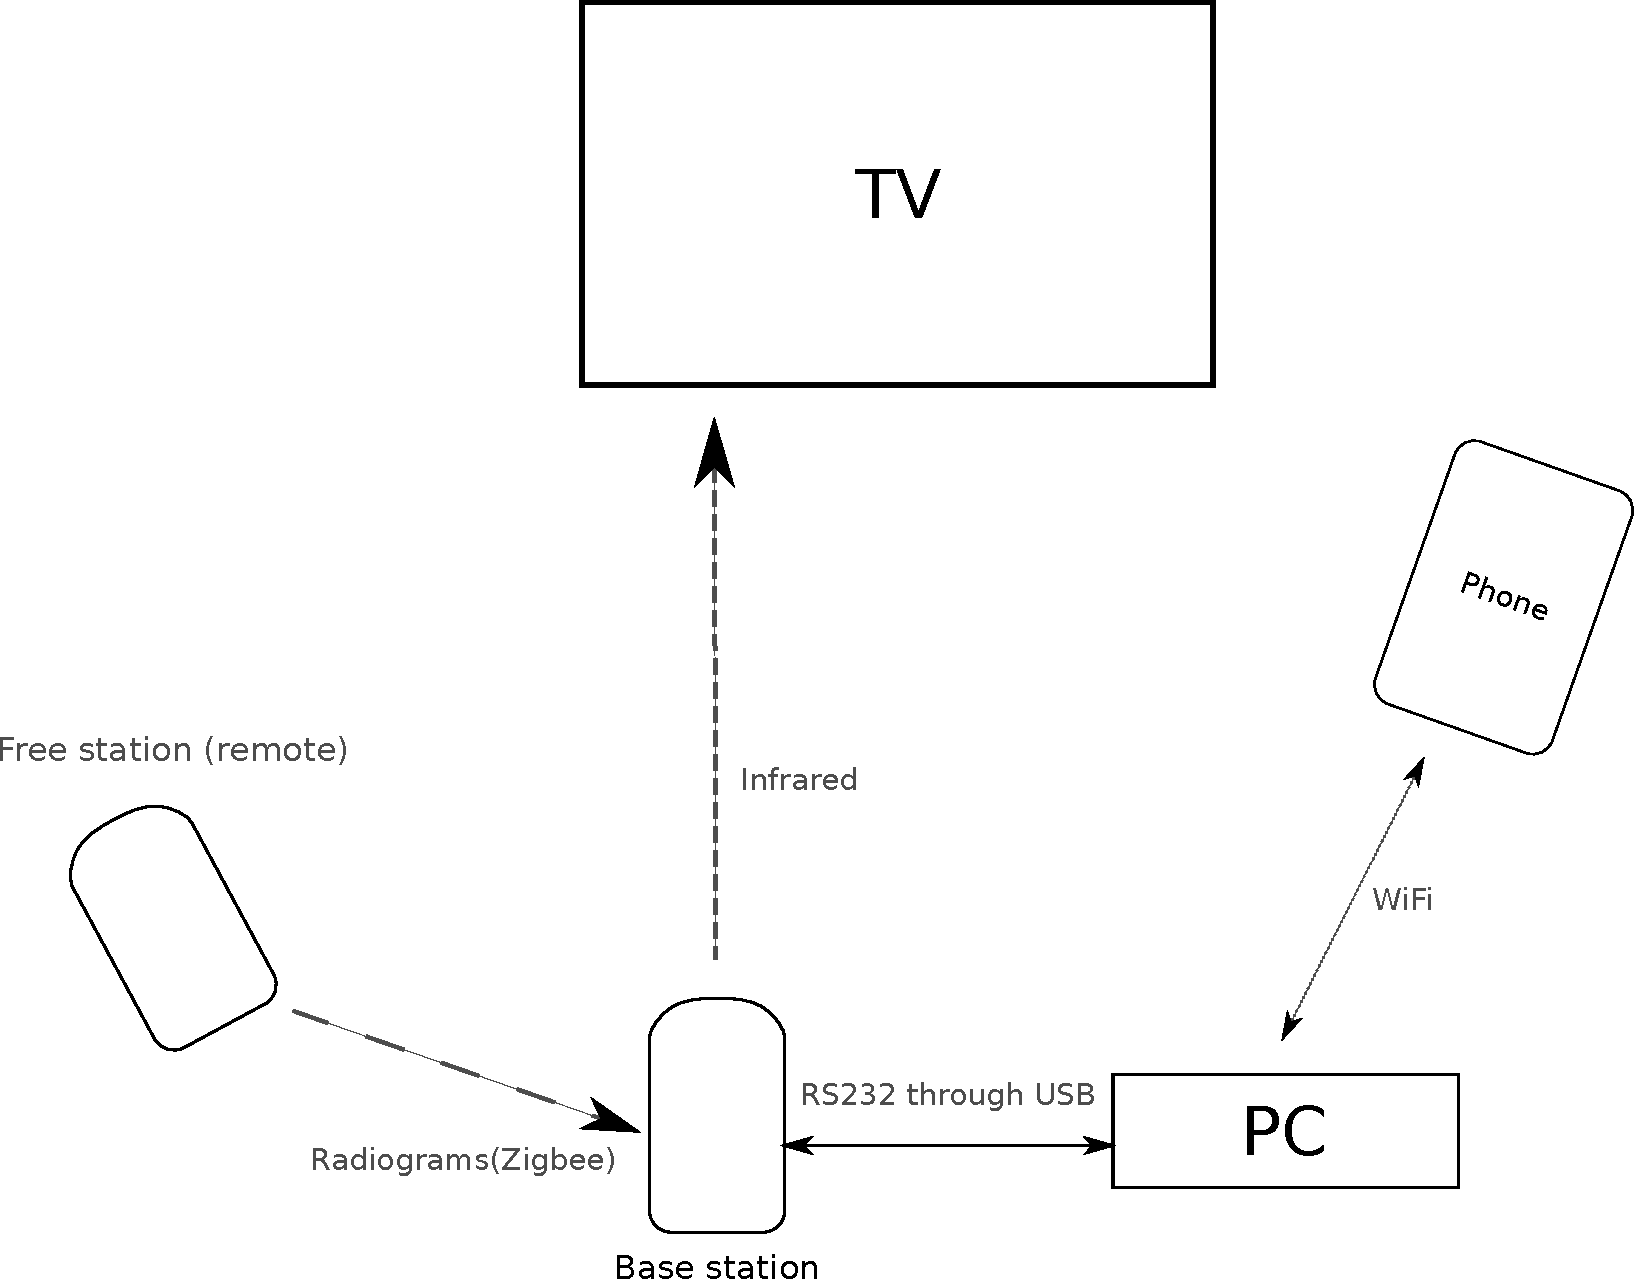
\includegraphics[scale=0.35]{stack.pdf}
  \end{center}
\end{frame}

\subsection{Remote}
\begin{frame}
  \begin{block}{User interface}
    \begin{itemize}
    \item uses the accelerometer as user input
    \item not as simple as it seems :/
    \item usable, but would need better algorithm
    \end{itemize}
  \end{block}
  \pause
  \begin{block}{Communication with the base station}
    \begin{itemize}
    \item really simple: a byte describing the command
    \item use radiograms
    \end{itemize}
  \end{block}
\end{frame}

\subsection{Base station}
\begin{frame}
  \begin{block}{Role 1: IR transmitter}
    One thread
    \begin{itemize}
    \item receives the radiograms from the free stations
    \item converts them to byte sequences corresponding to the TV's commands
    \item sends them through IR link
    \end{itemize}
  \end{block}

  \pause
  \begin{block}{Role 2: interfacing with the phone}
    A second thread wait for requests on serial line (through USB) and processes them or answers depending on the command
  \end{block}
\end{frame}

\begin{frame}
  \begin{block}{Command acceptance}
    \begin{itemize}
    \item the station stores a RSSI threshold
    \item if over, the command is accepted, otherwise it's dropped
    \item the RSSI threshold follows a $\propto \frac 1 t$ function, where $t$ is the time the last accepted command was received came
    \item {\bfseries problem} the RSSI varies \emph{heavily} in the same macro-conditions
    \end{itemize}
    $\Rightarrow$ theorically, the guy in the kitchen has to wait a loooong time to bother the girl in the sofa
  \end{block}
\pause
  \begin{block}{Parents/NSA/DGSE/GHCQ}
    The command emitted from a remote whose MAC is in the ``parents'' list override the system!
  \end{block}
\end{frame}


\subsection{Proxy}
\begin{frame}
  \begin{block}{Available communication}
    \begin{description}
    \item[Standard android phone] WiFi or Bluetooth
    \item[Sun SPOT] Zigbee or RS232 through USB
    \end{description}
  \end{block}
  To communicate or not to communicate, that is the question
  \pause
  \begin{block}{Solution}
    Use a proxy on the computer listening for requests on TCP socket then transmitting them through serial USB to the SPOT.

    However, the proxy isn't full duplex: no need for the SPOT to send something over TCP by itself.
  \end{block}
\end{frame}


\subsection{Android application}
\begin{frame}

\end{frame}

\begin{frame}[plain]{}
  \begin{center}
    {\bfseries \large Thanks for watching :)}\\
    \vspace{2cm}
    Any question?
  \end{center}
\end{frame}

\end{document}
